\section{Results of Case Studies}\label{sec:results}

Link to Appendix \ref{sec:additional-results}
\begin{itemize}
    \item Settings used.
\end{itemize}

\subsection{Glaucoma Data}

Figure \ref{fig:eye-results} displays the summary plot from the application of \texttt{GLaRe()} to the Glaucoma data.
PCA is to the most suitable latent feature representation method for this dataset because it achieves the qualifying criterion at $K=51$, whereas DWT and AE do not achieve the qualifying criterion for $K \leq 261$.
A grid of equally-spaced values from $1$ to $261$ in increments of $10$ was used for the latent feature dimensions. 
Although it was possible to use larger latent feature dimensions for the DWT and AE, the qualifying criterion was achieved for PCA at $K=51$ so it was deemed unnecessary.
The computation times for PCA, DWT and AE were $1.2$, $0.7$ and $69.4$ minutes, respectively.


\begin{figure}
    \centering
    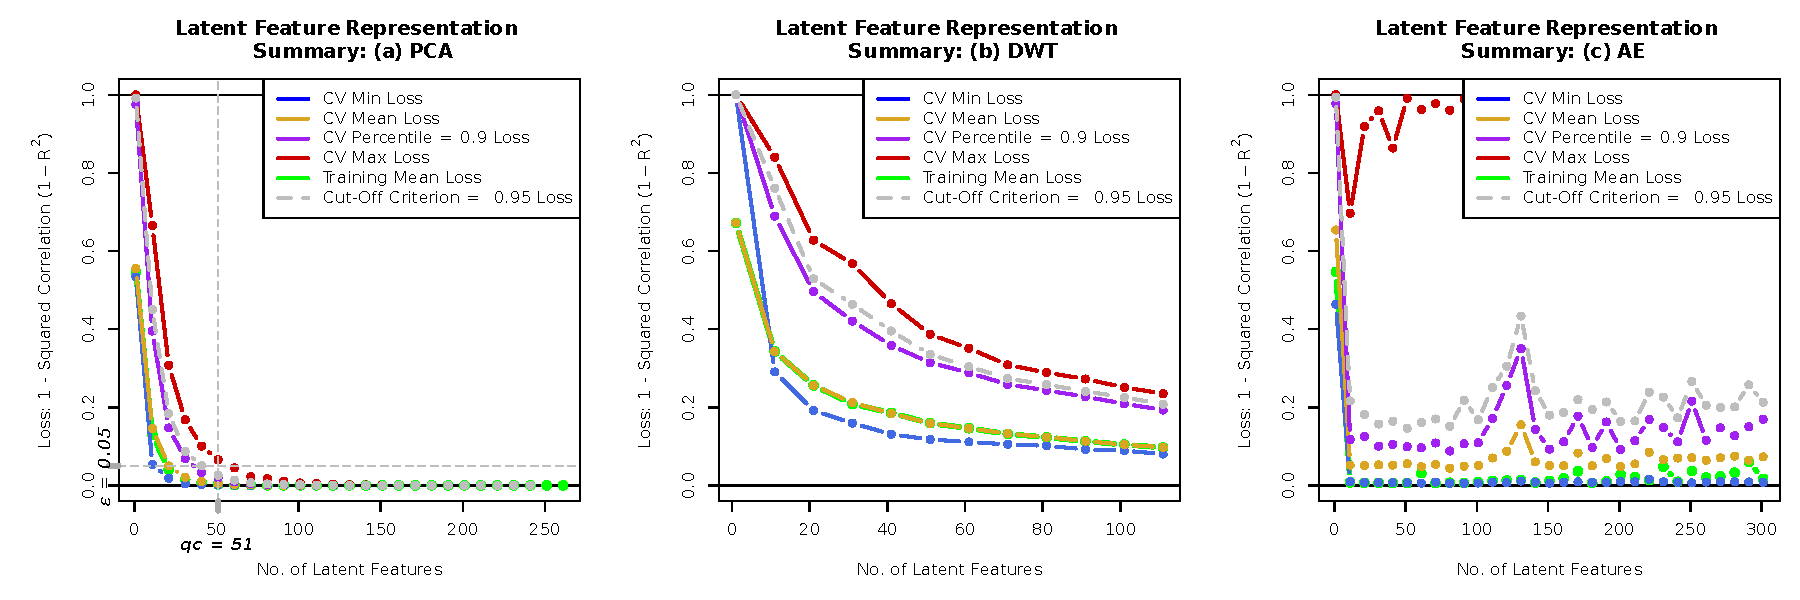
\includegraphics[width=1\textwidth]{figures/eye-results.pdf}
    \caption{Summary \texttt{GLaRe()} plot for the Glaucoma data. A grid of equally-spaced values from $1$ to $261$ in increments of $10$ was used for the latent feature dimensions.}
    \label{fig:eye-results}
\end{figure}

\subsection{Proteomic Gels Data}

\begin{figure}
    \centering
    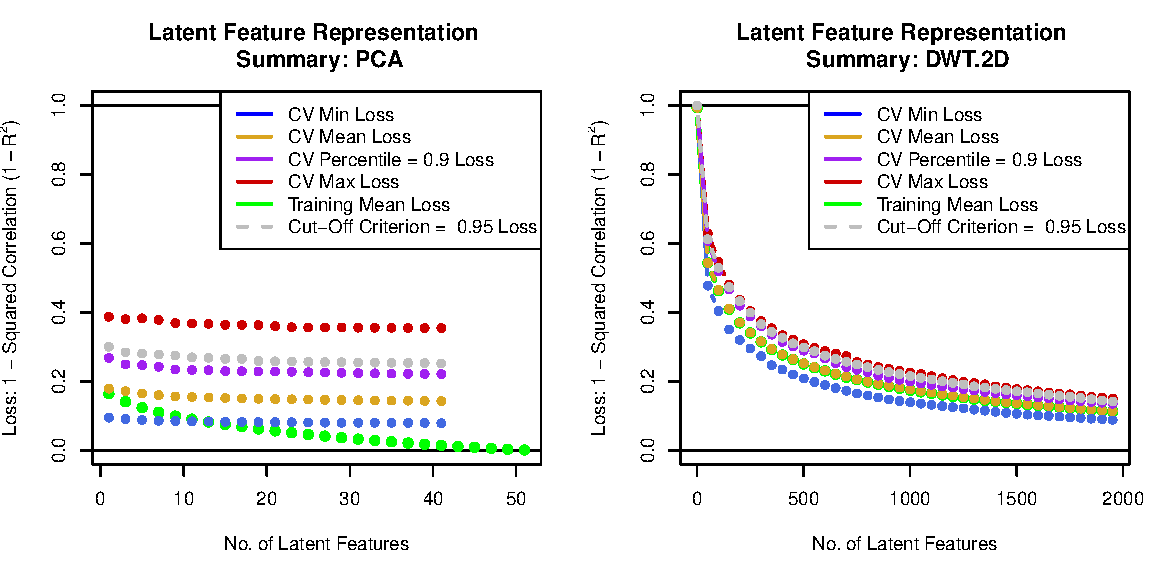
\includegraphics[width=1\linewidth]{figures/initial-gels.pdf}
    \caption{Preliminary results for the gels data.}
    \label{fig:enter-label}
\end{figure}


\subsection{MNIST Digits Data}


The computation times for PCA, DWT and AE were $X_1$, $X_2$ and $X_3$ minutes, respectively.



